% CHAPTER
\chapter{Composite polynomial approximation to \texorpdfstring{$\sqrt{x}$}{sqrt(x)}} \label{sqrtchapter}

\section{Zolotarev functions and matrix roots revisited}

The Zolotarev functions \eqref{zolotarevfn} have a diverse range of applications beyond the sign function, as seen in \cite[Section 3.7]{YujiZolotFreund} and \cite[Chapter 9]{akhiezer}. One particularly interesting feature is that best rational approximations to the square root on $[\delta^2,1]$, in the relative sense, are closely related to the Zolotarev functions: if
\[Z_{2r+1}(x;\delta) = x\dfrac{P_r(x^2)}{Q_r(x^2)}, \qquad P_r, Q_r \in \Pee_r,\]
then $Q_r(x)/P_r(x)$ is a rational best approximation to $\sqrt{x}$. Figure \ref{fig:ZOLOT_SQRT} illustrates the first few iterates for $\delta=0.1$. 

\bigskip{}

In recent literature, the Zolotarev functions have been used to construct iterations for computing the principal square root of a matrix \cite{Gawlik,ZolotGawlik}. The matrix square root is perhaps the most widely studied matrix function---a range of iterative procedures exist for the approximation of the matrix square root, and they are well-documented in \cite[Section 6.3]{Higham}. Beyond Newton's Method, we can also obtain a large class of iterations\footnote{Details can be found in the paper of Higham, Mackey, Mackey \& Tisseur \cite[Theorem 4.5]{highamgroups}.} for the principal square root from the matrix sign function, by means of the identity
\[\sgn\left(\begin{bmatrix} 0 & A \\ I & 0 \end{bmatrix}\right)=\begin{bmatrix} 0 & A^{1/2} \\ A^{-1/2} & 0 \end{bmatrix},\]
first noted by Higham in \cite{HighamStable}. Clearly there are deep connections between the sign and square root functions, and we use the above observations as motivation for assesses the connection between $\sgn(x)$ and $\sqrt{x}$ in the setting of polynomial approximations. The following example relates their best approximations over previously considered intervals.

\begin{figure}[t!]
\centering
   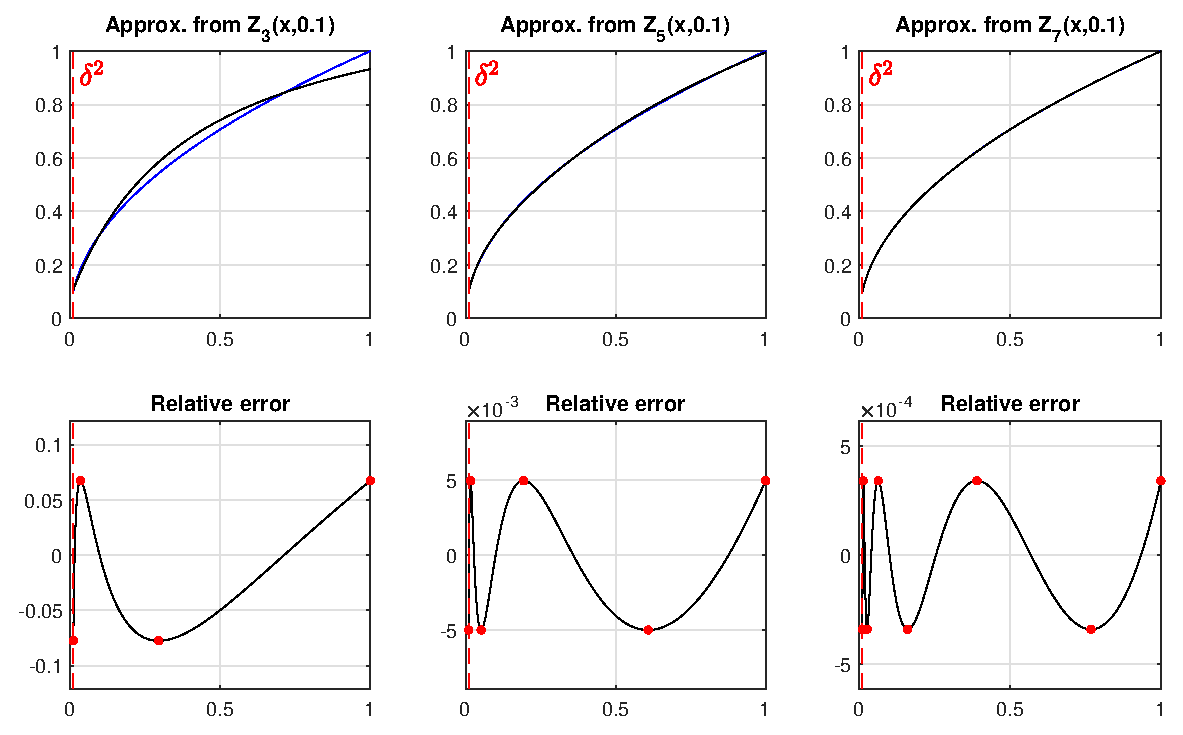
\includegraphics[width=\textwidth,height=\textheight,keepaspectratio]{figures/chapter_4/ZOLOTAREV_SQRT.eps}
   \caption{Approximations to $\sqrt{x}$ on $[\delta^2,1]$  for $\delta=0.03$, derived from the Zolotarev functions $Z_{2r+1}(x;\delta)$. The corresponding relative error is sketched below each plot, which equioscillates between $2r+2$ extrema in each case.}
   \label{fig:ZOLOT_SQRT}
\end{figure}

\begin{ex}\label{besties}
Consider the function $\sgn(x)$ on $X(\delta)$. Since $\sgn$ is odd, and $X(\delta)$ is symmetric about the origin, it follows by the remark after Lemma \ref{symm} that the best uniform polynomial approximation to $\sgn(x)$ on $X(\delta)$ is the best odd approximation $p^*(x)=xp(x^2)$ on $[\delta,1]$. Moreover, since $\sgn(x)=x/\sqrt{x^2}$ we can write the uniform error $\norm{\sgn-p^*}_{\infty,X(\delta)}$ as
\[\sup_{x\in [\delta,1]}|1 - xp(x^2)| = \sup_{x\in[\delta^2,1]}\left|\dfrac{xp(x)-\sqrt x}{\sqrt x}\right|.\]
That is, if the best uniform approximation to $\sgn(x)$ on $X(\delta)$ is $xp(x^2)$, then the best relative approximation to $\sqrt{x}$ on $[\delta^2,1]$ is $xp(x)$.
\end{ex}

Motivated by the connections between best approximations to $\sgn(x)$ and $\sqrt{x}$, this chapter attempts to use our scaled Newton-Schulz approximation to $\sgn(x)$ to generate a composite approximation to $\sqrt{x}$.

\section{Deriving an approximation from scaled Newton-Schulz iterates}

Recall the scaled Newton-Schulz approximation to $\sgn(x)$ on $X(\delta)$, given by
\begin{align}
    f_{k+1}(x)=\dfrac{f_k(x)}{2\xi_{k+1}}\left(3-\dfrac{f_k(x)^2}{\xi_{k+1}^2}\right), \qquad \xi_{k+1} = \sqrt{\dfrac{1+f_{k}(\delta)+f_{k}(\delta)^2}{3}}\label{forsqrt}
\end{align}
for $k\geq 0$, with initial guess $f_0(x)=x$. Here the $f_k$ approximate $C_k \sgn(x)$, where $C_k=(1+f_k(\delta))/2$. Each $f_k$ is an odd function, hence by Lemma \ref{symm} we can write $f_k(x)=xh_k(x^2)$ for some polynomial $h_k$. This observation allows us to derive a square root approximation, which we illustrate in Figure \ref{fig:compsqrt3}.

\begin{thm}
Let $\delta \in (0,1)$, $f_k \in \Pee_{(k,3)}^{\text{comp}}$ be the scaled Newton-Schulz iteration to $C_k \sgn (x)$ defined by \eqref{forsqrt}, and $E_k$ be the maximum uniform error. Writing $f_k(x)=xh_k(x^2)$, the iterates $F_k(x)=xh_k(x)$ provide a composite approximation 
\[F_{k+1}(x) = \dfrac{F_k(x)}{2\xi_{k+1}}\left(3-\dfrac{F_k(x)^2}{x\xi_{k+1}^2}\right), \qquad \xi_k = \sqrt{\dfrac{\delta^2+\delta F_{k-1}(\delta^2) + F_{k-1}(\delta^2)^2}{3\delta^2}} \]
to $\sqrt{x}$, for which
\[\norm{F_k - C_k\sqrt{x}}_{\infty,[\delta^2,1]} \leq E_k.\]
\end{thm}

\begin{proof}
The error bound follows from the fact that
\begin{align*}
    \norm{\sgn-C_k^{-1}f_k}_{\infty,X(\delta)}&= \norm{\dfrac{C_k x\sgn-xf_k}{C_k x}}_{\infty,X(\delta)}\\
    &=\norm{\dfrac{C_k\sqrt{x}-F_k}{C_k\sqrt{x}}}_{\infty,[\delta^2,1]}\\
    & \geq C_k^{-1} \norm{C_k\sqrt{x}-F_k}_{\infty,[\delta^2,1]},
\end{align*}
similar to Example \ref{besties}. To obtain a recursion for the $F_k$, we first note that
\[F_k(\delta^2)=\delta^2 h_k(\delta^2) = \delta f_k(\delta),\]
so we can rewrite $\xi_k$ in terms of the $F_{k-1}$, namely
\[\xi_k = \sqrt{\dfrac{\delta^2+\delta F_{k-1}(\delta^2) + F_{k-1}(\delta^2)^2}{3\delta^2}}.\]
We can derive a sequence for the $F_k$, since by \eqref{forsqrt} we have
\[xh_{k+1}(x^2)=\dfrac{xh_k(x^2)}{2\xi_{k+1}}\left(3-\dfrac{x^2h_k(x^2)^2}{\xi_{k+1}^2}\right),\]
hence a recursion for the $h_k$ is given by
\[h_{k+1}(x) = \dfrac{h_k(x)}{2\xi_{k+1}}\left(3-\dfrac{xh_k(x)^2}{\xi_{k+1}^2}\right).\]
Multiplying by $x$ gives
\begin{align}
    F_{k+1}(x) = \dfrac{F_k(x)}{2\xi_{k+1}}\left(3-\dfrac{F_k(x)^2}{x\xi_{k+1}^2}\right), \label{comprelsqrt}
\end{align}
as required.
\end{proof}

\begin{figure}[t!]
\centering
   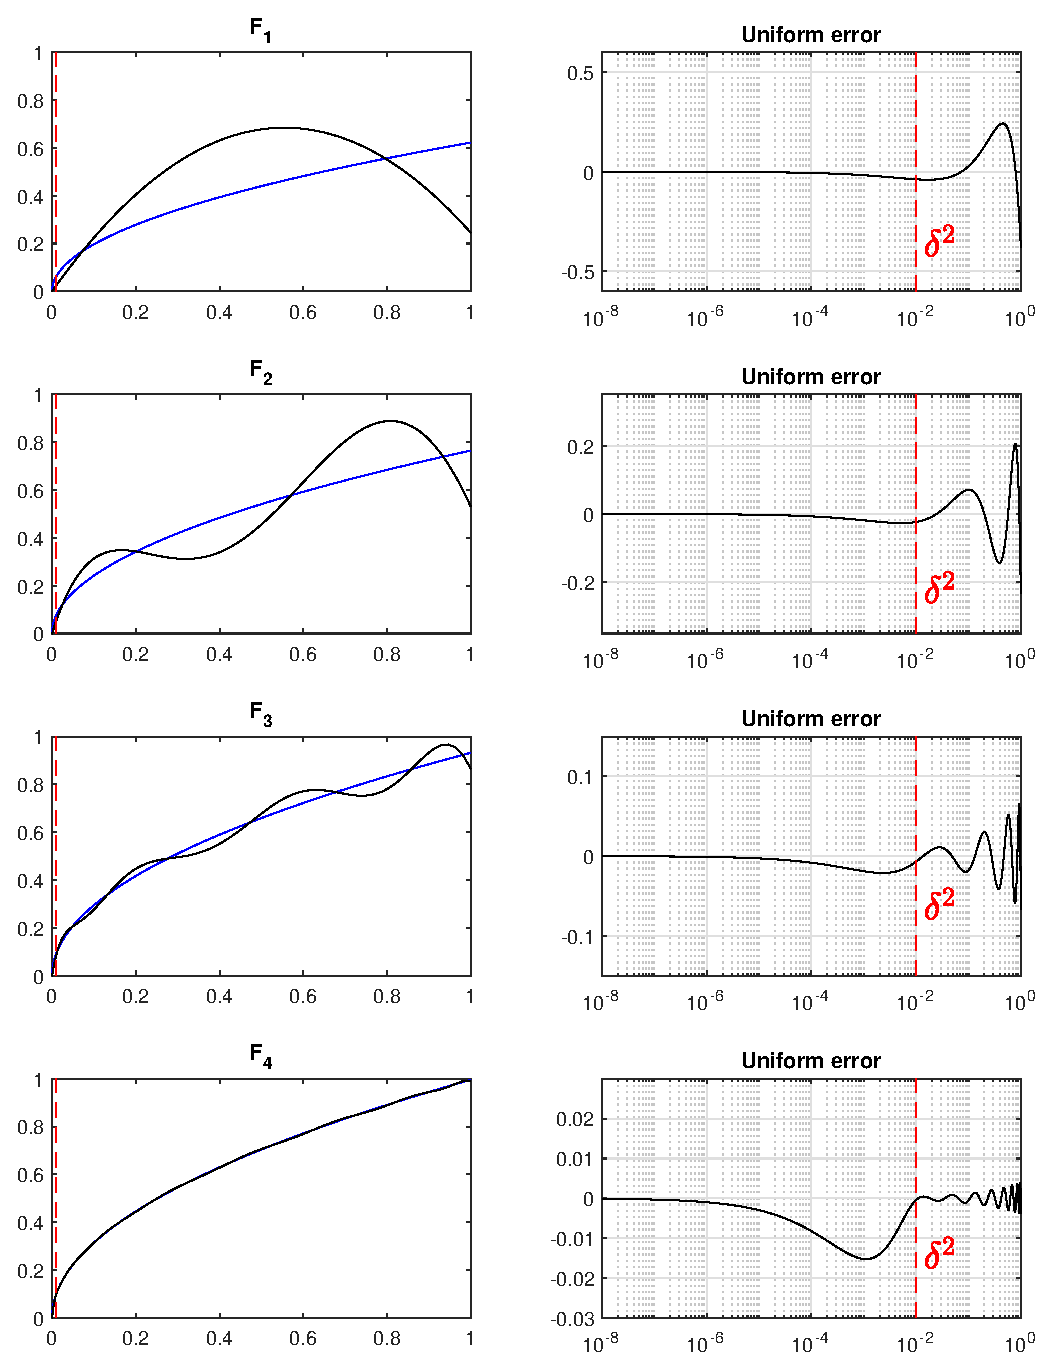
\includegraphics[width=\textwidth,height=\textheight,keepaspectratio]{figures/chapter_4/COMPSQRT_4ITERS_UNIF.eps}
   \caption{Composite polynomial approximations $F_k$ (black) to $C_k\sqrt{x}$ (blue) on $[0,1]$, choosing $\delta=0.1$ (red dashed line). The uniform errors are plotted beside each iteration. On $[\delta^2,1]$, the relative error will be identical to the uniform error the scaled Newton-Schulz iterates to the sign function on $X(\delta)$.}
   \label{fig:compsqrt3}
\end{figure}

\begin{rmk}
For any initial guess $F_0$ divisible by $x$, it follows inductively that $F_k$ is a polynomial for all $k$. This is a non-pure composite approximation to $C_k\sqrt{x}$ on $[\delta^2,1]$ in the relative sense, and the error analysis will thus fall largely in line with that of the previous chapter. Furthermore, the iteration \eqref{comprelsqrt} can be seen as a scaled version of the Alternative Newton iterates \eqref{altnewt} considered in the preliminary discussion, where once again the iteration function $G_k$ is such that $x$ is replaced by $x\xi_k^{-1}$. As such, we will refer to these as \textit{scaled Alternative Newton} iterates to $\sqrt{x}$.
\end{rmk}

\section{Observations of the scaled Alternative Newton iterates}

On the interval $[\delta^2,1]$, our convergence analysis follows largely as in the previous chapter due to Theorem 4.2. A natural question to ask is how convergence differs when considering the $F_k$ on the whole interval $[0,1]$. In particular, if we are allowed at most $k$ iterations, what is the value of $\delta$ that we should choose to minimise the error? The answer to this question is far from obvious, as Figures \ref{fig:scaled_alt1}-\ref{fig:scaled_alt4} illustrate. These figures compare the maximum error in the unscaled and scaled Alternative Newton iterates, alongside the standard Newton iteration. As we might have expected, the Newton iteration eventually outperforms the alternative iterations for all choices of $\delta$. What is unexpected is that for sufficiently small values of $\delta$, the scaled Alternative Newton approximation can even perform better than Newton's method. For instance, if we allow ourselves 10 iterations, it is more efficient to use our approximation with $\delta=0.001$ with the standard Newton iterates.

\begin{figure}[t!]
\centering
   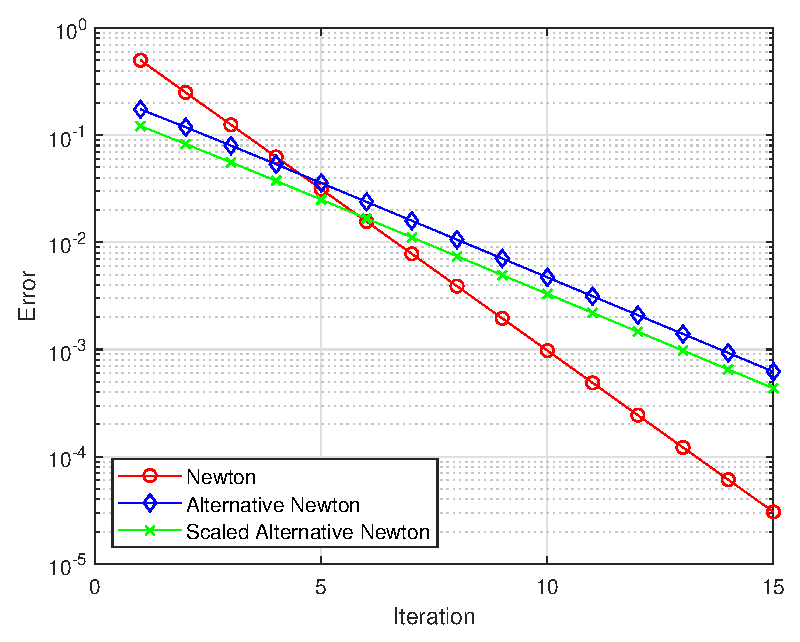
\includegraphics[width=0.7\textwidth,height=0.7\textheight,keepaspectratio]{figures/chapter_4/AN_vs_SAN_0p5.eps}
   \caption{Comparison of the error in Newton, Alternative Newton and scaled Alternative Newton iterates to $\sqrt{x}$ on $[0,1]$, with a choice of $\delta=0.5$.}
   \label{fig:scaled_alt1}
\end{figure}

\begin{figure}[t!]
\centering
   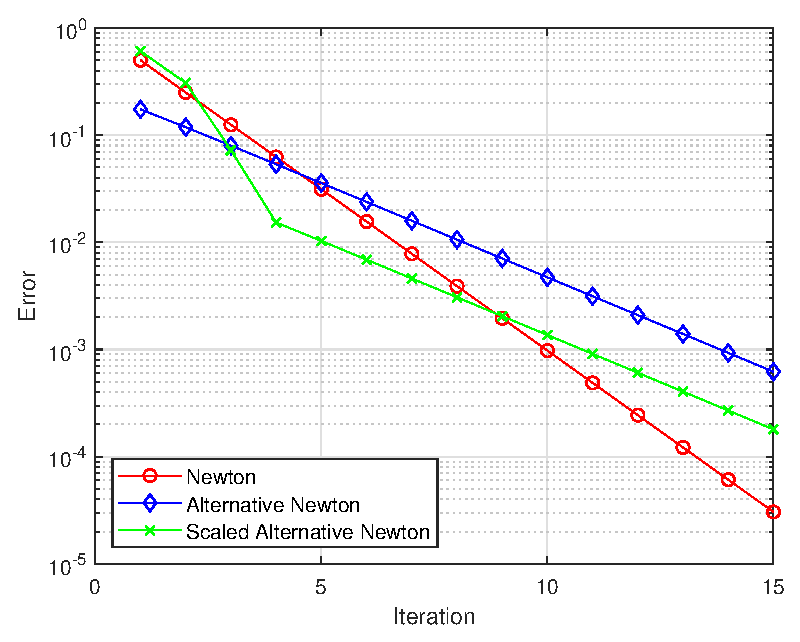
\includegraphics[width=0.7\textwidth,height=0.7\textheight,keepaspectratio]{figures/chapter_4/AN_vs_SAN_0p1.eps}
   \caption{Comparison of the error in Newton, Alternative Newton and scaled Alternative Newton iterates to $\sqrt{x}$ on $[0,1]$, with a choice of $\delta=0.1$.}
   \label{fig:scaled_alt2}
\end{figure}

\begin{figure}[t!]
\centering
   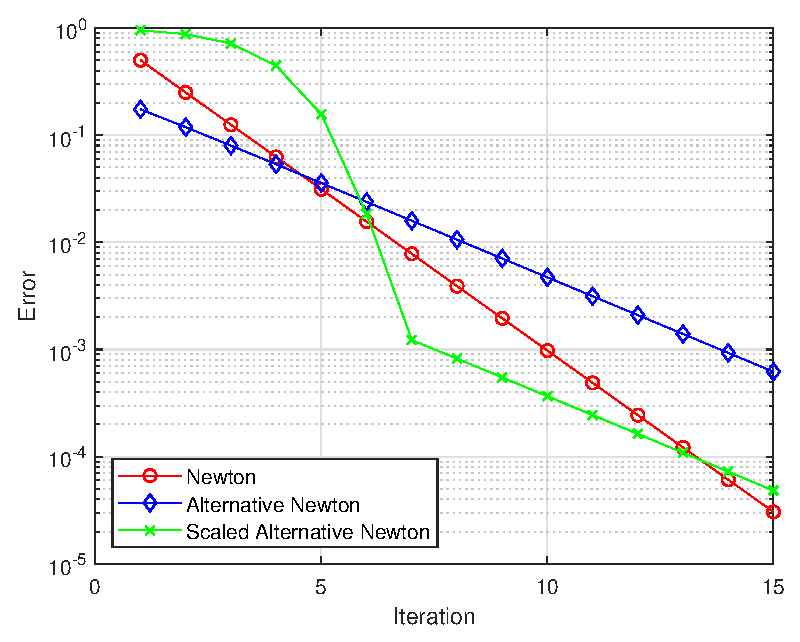
\includegraphics[width=0.7\textwidth,height=0.7\textheight,keepaspectratio]{figures/chapter_4/AN_vs_SAN_0p01.eps}
   \caption{Comparison of the error in Newton, Alternative Newton and scaled Alternative Newton iterates to $\sqrt{x}$ on $[0,1]$, with a choice of $\delta=0.01$.}
   \label{fig:scaled_alt3}
\end{figure}

\begin{figure}[t!]
\centering
   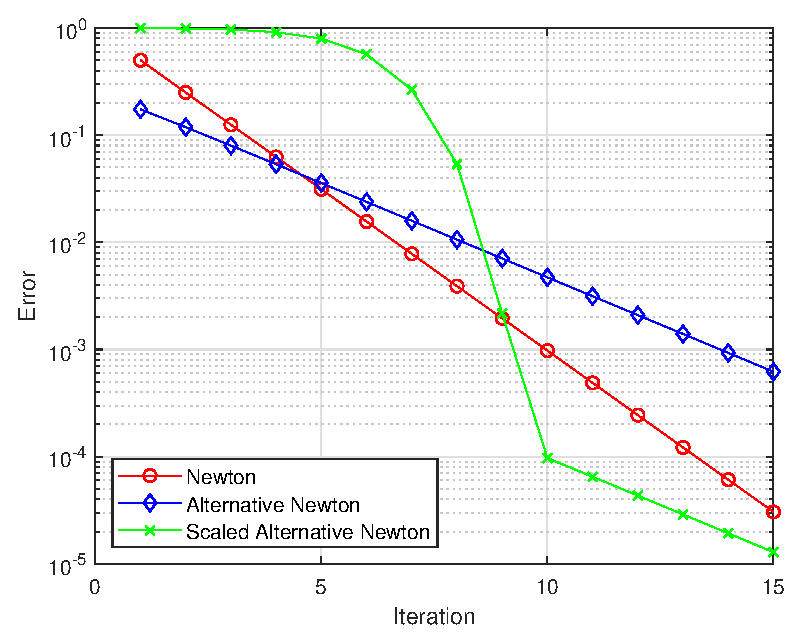
\includegraphics[width=0.7\textwidth,height=0.7\textheight,keepaspectratio]{figures/chapter_4/AN_vs_SAN_0p001.eps}
   \caption{Comparison of the error in Newton, Alternative Newton and scaled Alternative Newton iterates to $\sqrt{x}$ on $[0,1]$, with a choice of $\delta=0.001$.}
   \label{fig:scaled_alt4}
\end{figure}